%!TEX root = ../thesis.tex
% ******************************* Thesis Appendix B ********************************

\begin{figure}[htbp!] 
\centering    
    \includegraphics[width=1\textwidth]{Chapter3/Figs/Supps/FigureS1_Differences_in_development_embryos.pdf}
\caption{\textit{Marchantia} embryos develop at different rates in different environmental conditions}
\label{fig:embryo_diff}
\captionsetup{font=small}
    \caption*{DAPI stained \textit{Marchantia} embryos at 10 days after fertilisation (first row), and 12 days after fertilisation (second and third rows) showing different developmental stages. Scale bar 10 $\mu$m.}
\end{figure}

\begin{figure}[htbp!] 
\centering    
    \includegraphics[width=1\textwidth]{Chapter3/Figs/Supps/FigureS2_Fixing_MpSUN_trials.pdf}
\caption{Fixing and staining results of wild type (first row) ECPro::MpSUN-GFP embryos (third row) and gemmae (second row). Scale bar 10 $\mu$m.}
\label{fig:MpSUN}
\captionsetup{font=small}
    \caption*{}
\end{figure}

\begin{figure}[htbp!] 
\centering    
    \includegraphics[width=1\textwidth]{Chapter3/Figs/Supps/FigureS3_enzyme_tests.pdf}
\caption{Fixing and staining results of embryos after treatment with cell wall digesting enzymes}
\label{fig:enzyme_tests}
\captionsetup{font=small}
    \caption*{Scale bar 10 $\mu$m.}
\end{figure}

\begin{landscape}
\begin{figure}[htbp!] 
\centering    
    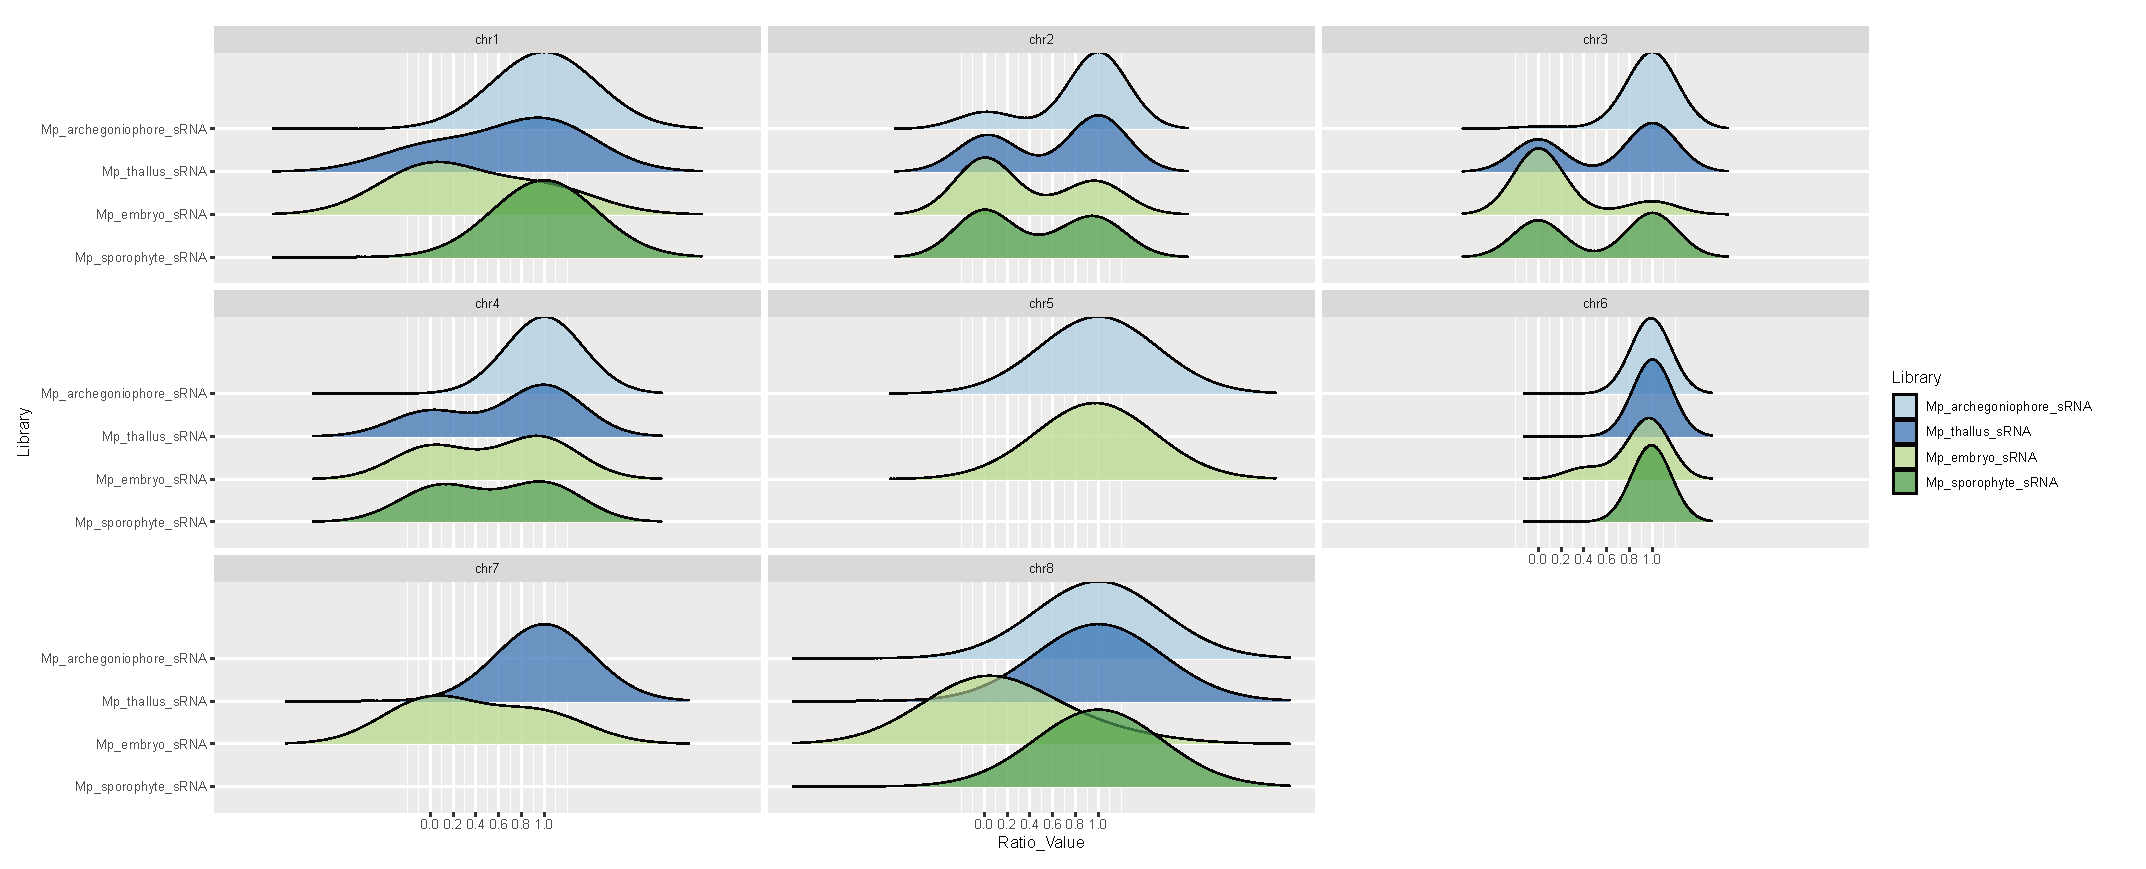
\includegraphics[width=1.7\textwidth]{Chapter3/Figs/Supps/FigureS_chrom_ridge_plot.pdf}
\caption{Ridge plot to show the SNP ratio of sRNAs in archegoniophores, thallus, embryo and sporophyte, faceted by chromosome.}
\label{fig:chrom_ridge}
\captionsetup{font=small}
    \caption*{}
\end{figure}
\end{landscape}

\begin{figure}[htbp!] 
\centering    
    \includegraphics[width=1\textwidth]{Chapter3/Figs/Supps/0vs3_mismatch_Arabidopsis.pdf}
\caption{Violin/box plots of the abundance of 24nt sRNAs in seedling, meiocyte, sperm cell, sperm nucleus and pollen in \textit{Arabidopsis} mapped with 0 (dark green) and 3 (light green) mismatches}
\label{fig:At_0v3}
\captionsetup{font=small}
    \caption*{}
\end{figure}

\begin{figure}[htbp!] 
\centering    
    \includegraphics[width=1\textwidth]{Chapter3/Figs/Supps/0v3_mismatch_Marchantia.pdf}
\caption{Violin/box plots of the abundance of 24nt sRNAs in the thallus, embryo and sporophyte in \textit{Marchantia} mapped with 0 (dark green) and 3 (light green) mismatches}
\label{fig:Mp_0v3}
\captionsetup{font=small}
    \caption*{}
\end{figure}

\begin{figure}[htbp!] 
\centering    
    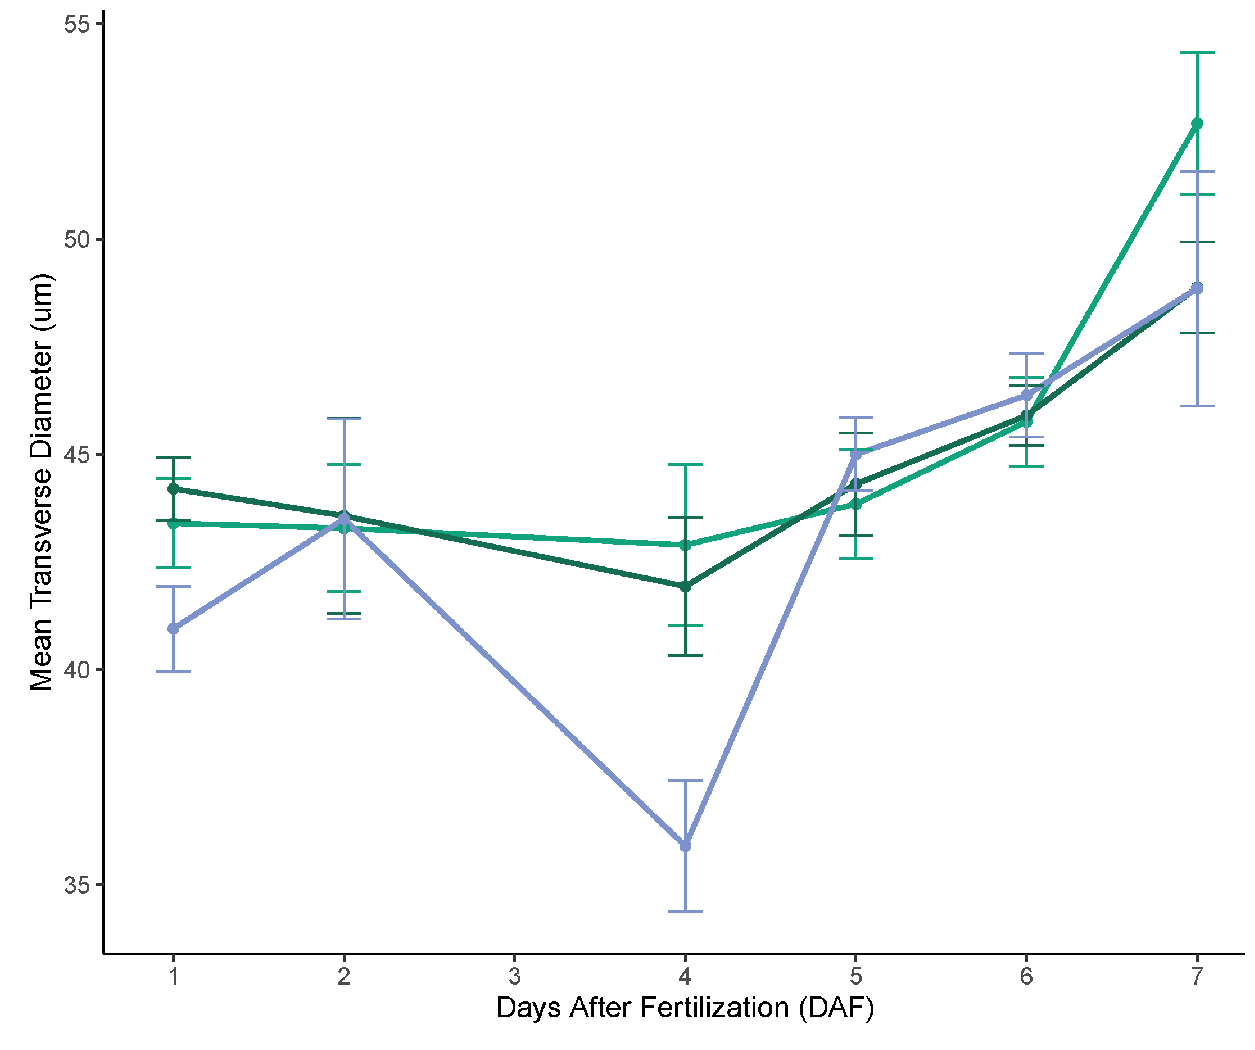
\includegraphics[width=1\textwidth]{Chapter3/Figs/Supps/FigureS4_transverse_diameter.pdf}
\caption{Line graph that shows the transverse diameter of embryos fertilised by wild type (blue) or 2 independent 4mC mutant (green) sperm.}
\label{fig:transverse_diameter}
\captionsetup{font=small}
    \caption*{}
\end{figure}

\begin{figure}[htbp!] 
\centering    
    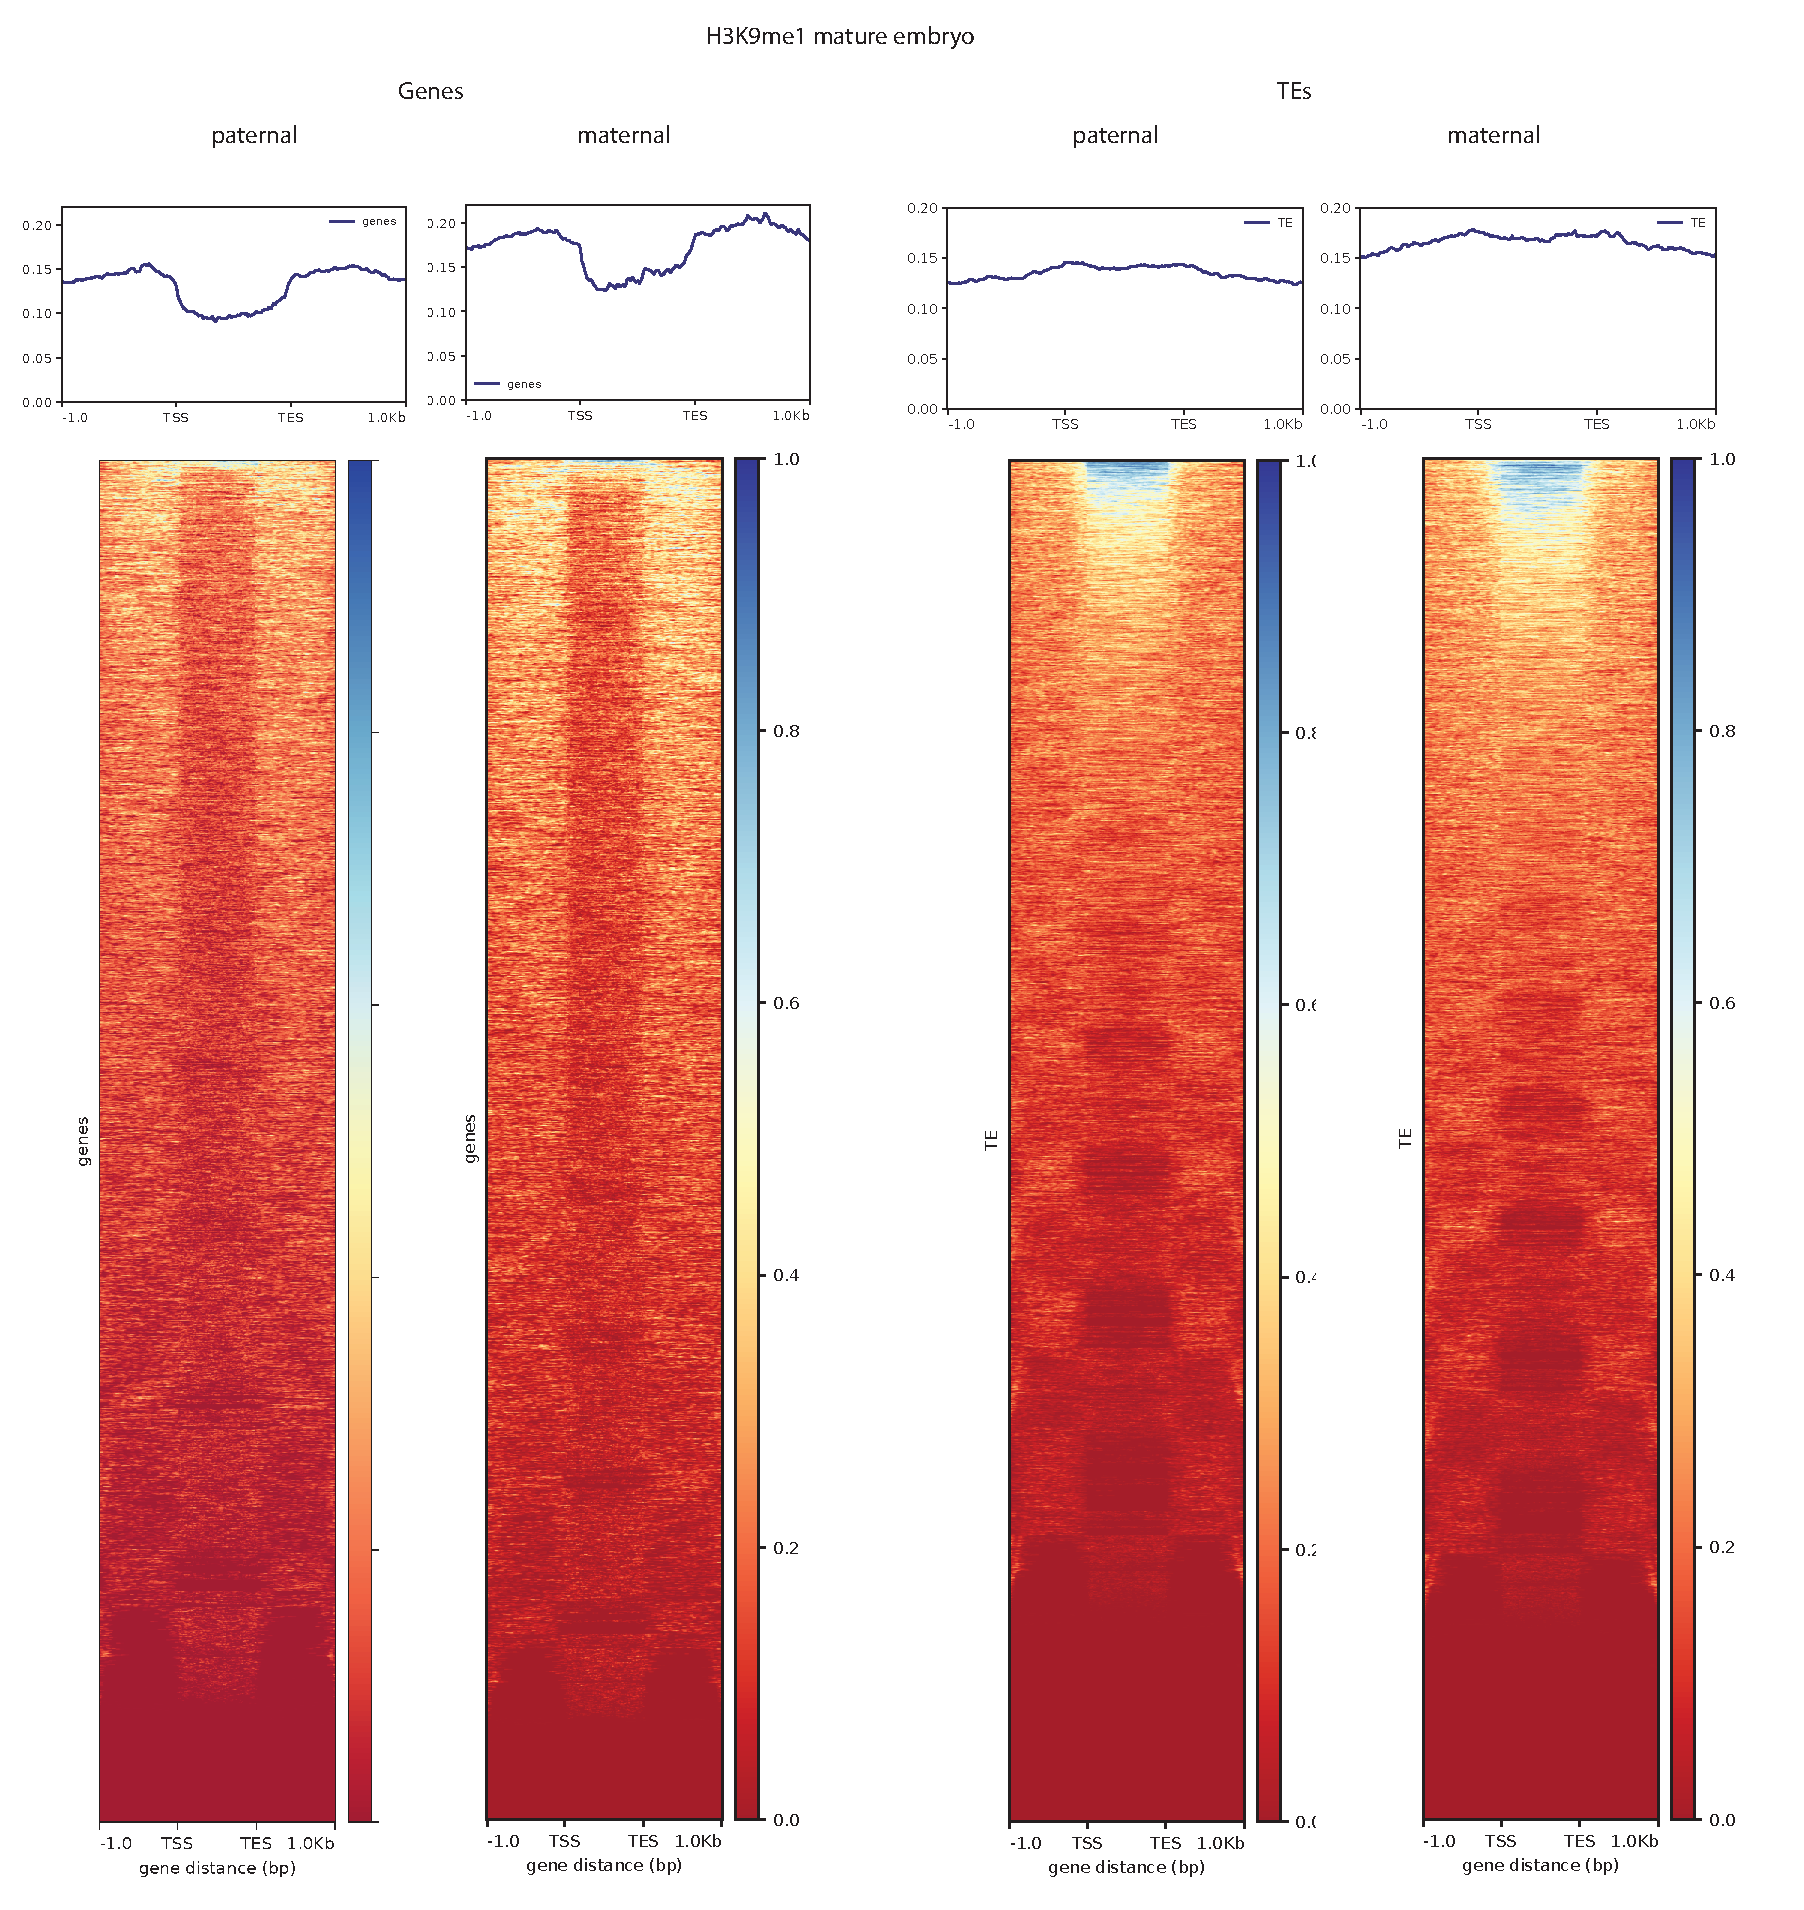
\includegraphics[width=1\textwidth]{Chapter3/Figs/Supps/FigureS5_H3k9me1.pdf}
\caption{H3K9me1 over genes and TEs is not associated with the paternal genome}
\label{fig:h3k8me1}
\captionsetup{font=small}
    \caption*{Heatmap showing the relative distribution of H3K9me1 over genes and TEs associated with paternal or maternal genomes. Data presented is from \cite{RN160}}
\end{figure}

\begin{figure}[htbp!] 
\centering    
    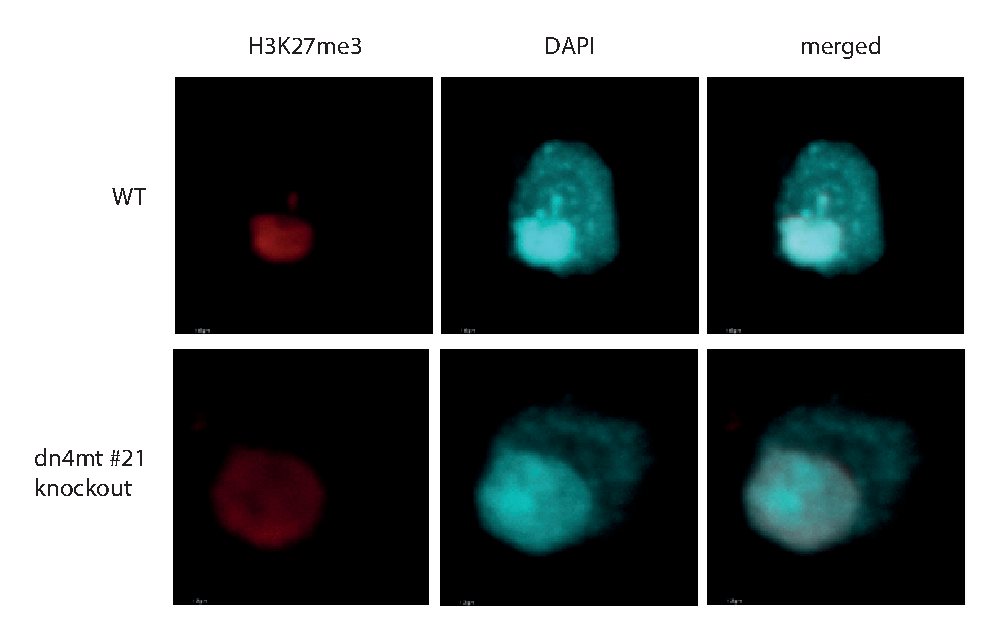
\includegraphics[width=1\textwidth]{Chapter3/Figs/Supps/FigureS1_immunostaining.pdf}
\caption{Immunostaining of H3K27me3 in 13 DAF embryos fertilised by wild type and dn4mt1 \#21 knockout sperm }
\label{fig:immuno}
\captionsetup{font=small}
    \caption*{}
\end{figure}

\begin{table}[htbp]
    \centering
    \scriptsize % Keep the font size as scriptsize
    \caption{Primers used for nuclear reporter line cloning}
    \label{table:reporter_primers}
    \begin{tabular}{>{\raggedright\arraybackslash}p{3.4cm} >{\raggedright\arraybackslash}p{2.8cm} >{\raggedright\arraybackslash}p{4.7cm} >{\raggedright\arraybackslash}p{1.9cm}}
    \toprule
    Construct Target & Name & Sequence & Purpose \\
    \midrule
    pMpGWB115 or pMpGWB116 & attB1-fluo-NLS-attB2-f1 & \seqsplit{GGGGACAAGTTTGTACAAAAAAGCAGGCTTAATGGTGAGCAAGGGCGAG} & citrine/tdTom insert + attB sites \\
    pMpGWB115 or pMpGWB117 & attB1-fluo-NLS-attB2-r1 & \seqsplit{GGGGACCACTTTGTACAAGAAAGCTGGGTTCTATCCTCCAACCTTTCTCTTCTTCTTAGG} & citrine/tdTom insert + attB sites \\
    \midrule
    pMpGWB102-Citrine-NLS \& pMpGWB103-Citrine-NLS entry clones (pDONR221) & citrine-ent-seq-f1 & \seqsplit{TTAATGGTGAGCAAGGGC} & Entry clone sequencing \\
    & citrine-ent-seq-r1 & \seqsplit{TGGGTTCTATCCTCCAACC} & Entry clone sequencing \\
    pMpGWB102-tdTom-NLS \& pMpGWB103-tdTom-NLS entry clones (pDONR221) & tdTom-ent-seq-f1 & \seqsplit{AGGCTTAATGGTGAGCAAG} & Entry clone sequencing \\
    & tdTom-ent-seq-r1 & \seqsplit{GGGTTCTATCCTCCAACC} & Entry clone sequencing \\
    \midrule
    pMpGWB102-Citrine-NLS & 102-citrine-exp-seq-f1 & \seqsplit{TTGGAGAGAACACGGG} & Expression clone sequencing \\
    & 102-citrine-exp-seq-r1 & \seqsplit{CTGGGTTCTATCCTCCAAC} & Expression clone sequencing \\
    pMpGWB102-tdTom-NLS & 102-tdTom-exp-seq-f1 & \seqsplit{AGAGAACACGGGGGACTC} & Expression clone sequencing \\
    & 102-tdTom-exp-seq-r2 & \seqsplit{TCGGAGGAGGCGGTG} & Expression clone sequencing \\
    & 102-tdTom-exp-seq-r1 & \seqsplit{ACAAGAAAGCTGGGTTCTATCCTC} & Expression clone sequencing \\
    \midrule
    pMpGWB103-Citrine-NLS & 103-citrine-exp-seq-f1 & \seqsplit{CCTCGAGCGAGTGATTTTTTAGG} & Expression clone sequencing \\
    & 103-citrine-exp-seq-r1 & \seqsplit{GGGTTCTATCCTCCAACCTTTC} & Expression clone sequencing \\
    pMpGWB103-tdTom-NLS & 103-tdTom-exp-seq-f1 & \seqsplit{ATTTCGCTAATCATTCCCTAATTTC} & Expression clone sequencing \\
    & 103-tdTom-exp-seq-r2 & \seqsplit{CGGCCATGTTGTTGTC} & Expression clone sequencing \\
    & 103-tdTom-exp-seq-r1 & \seqsplit{AAGAAAGCTGGGTTCTATCC} & Expression clone sequencing \\
    \bottomrule
    \end{tabular}
\end{table}

\begin{figure}[htbp]
\centering
\includegraphics[width=1\textwidth]{Appendix2/Figs/1-expression-clone-pMpGWB102(35S)+citrine Map.pdf}
\caption{Plasmid map of pMpGWB102(35S)-citrine-NLS}
\label{fig:35S_citrine_map}
\end{figure}

\begin{figure}[htbp]
\centering
\includegraphics[width=1\textwidth]{Appendix2/Figs/2-expression-clone-pMpGWB102(35S)+tdTomato Map.pdf}
\caption{Plasmid map of pMpGWB102(35S)-tdTomato-NLS}
\label{fig:35S_tdTomato_map}
\end{figure}

\begin{figure}[htbp]
\centering
\includegraphics[width=1\textwidth]{Appendix2/Figs/3-expression-clone-pGWB103(EFalpha)+citrine Map.pdf}
\caption{Plasmid map of pMpGWB103(\textit{EF1$\alpha$})-citrine-NLS}
\label{fig:EFalpha_citrine_map}
\end{figure}

\begin{figure}[htbp]
\centering
\includegraphics[width=1\textwidth]{Appendix2/Figs/4-expression-clone-pGWB103(EFalpha)+tdTomato Map.pdf}
\caption{Plasmid map of pMpGWB102(\textit{EF1$\alpha$})-tdTomato-NLS}
\label{fig:EFalpha_tdTomato_map}
\end{figure}

\begin{table}[htbp]
\centering
\begin{tabular}{|p{6cm}|p{3cm}|p{4cm}|} % Same column widths as the second part
\hline
\textbf{Line name} &  & \textbf{Source} \\
\hline
Tak-1 & & Feng Lab \\
Tak-2 & & Feng Lab \\
Cam-2 & & Feng Lab \\
35s::tdTomato-NLS (Tak-1 male, WT female backgrounds) & & Feng Lab (constructed by JT) \\
\textit{EF1$\alpha$}::citrine-NLS (Tak-1 male, WT female backgrounds) & & Feng Lab (constructed by JT) \\
\textit{EF1$\alpha$}::tdTomato-NLS (Ta-k1 male, WT female backgrounds) & & Feng Lab (constructed by JT) \\
\textit{dn4mt1} k.o. \#6 & & Feng Lab \cite{RN189} \\
\textit{dn4mt1} k.o. \#21 & & Feng Lab \cite{RN189} \\
\textit{dnmt3b} k.o. & & Feng Lab \cite{RN189} \\
\textit{cmta} k.o. & & Feng Lab \cite{RN189} \\
\hline
\end{tabular}
\begin{tabular}{|p{6cm}|p{3cm}|p{4cm}|}
\hline
\textbf{Library name} & \textbf{Library type} & \textbf{Source} \\
\hline
WT sperm & EM-seq & Feng Lab (constructed by JT) \\
WT sperm & AMD-seq & Feng Lab (constructed by JT) \\
WT sperm & AMD-seq & Feng Lab \\
\textit{dn4mt1} k.o. sperm & AMD-seq & Feng Lab \\
14 DAF embryo & AMD-seq & Feng Lab (constructed by JT) \\
7-8 DAF embryo & A3A-sc-BS-seq & Feng Lab (constructed by JT) \\
\hline
Archegoniophore & sRNA & \cite{RN308} \\
Embryo & sRNA & Feng Lab \\
Sporophyte & sRNA & Feng Lab \\
Thallus & sRNA & Feng Lab \\
\hline
Embryo & BS-seq & Feng Lab \\
Sporophyte & BS-seq & Feng Lab \\
Thallus & BS-seq & Feng Lab \\
Embryo & H3K27me3 CUT\&RUN & \cite{RN160} \\
Embryo & H3K9me1 CUT\&RUN & \cite{RN160} \\
\hline
\end{tabular}
\caption{Table depicting the line names, library types, and sources of the data presented in this chapter.}
\label{ch3:workbyothers}
\end{table}


